\chapter{The Distance Matching Principle}

\begin{goals}
\begin{itemize}
    \item Propose a core principle: good parameterization matches distances
    \item See how this explains known successes
    \item Understand what remains to be formalized
\end{itemize}
\end{goals}

\section{The Observation}

Why is linear regression optimal for linear functions?

\begin{enumerate}
    \item Expressiveness: linear model can represent all linear functions
    \item No redundancy: different parameters give different functions
    \item Convex optimization: unique global minimum
    \item Gauss-Markov: statistically optimal (BLUE)
\end{enumerate}

But there's a deeper reason unifying all of these:

\begin{keyinsight}
In linear regression, parameter distance is proportional to function distance.

If $\theta_1$ and $\theta_2$ are close in $\mathbb{R}^{d+1}$, then $f_{\theta_1}$ and $f_{\theta_2}$ are close as functions.

The parameterization ``matches'' the function space geometry.
\end{keyinsight}

\section{Distance Matching}

\begin{definition}[Informal]
A parameterization $\gamma: \Theta \to \mathcal{F}$ \textbf{matches distances} if:
\[
d_\Theta(\theta_1, \theta_2) \approx c \cdot d_{\mathcal{F}}(\gamma(\theta_1), \gamma(\theta_2))
\]
for some constant $c > 0$.
\end{definition}

Strict version: $\gamma$ is an \textbf{isometry} (distance-preserving map).

Weak version: distances are \textbf{proportional} (up to bounded distortion).

\section{Why Distance Matching Helps Optimization}

Gradient descent moves in the steepest direction in parameter space.

\textbf{If distances match}: steepest in $\Theta$ = steepest in $\mathcal{F}$. Gradient descent does the ``right thing.''

\textbf{If distances don't match}:
\begin{itemize}
    \item Some directions in $\Theta$: move far, function barely changes (redundant)
    \item Some directions in $\Theta$: move little, function changes a lot (sensitive)
    \item Gradient descent zigzags, wastes effort
\end{itemize}

\section{Case Studies}

\subsection{Linear Regression: Perfect Match}

\begin{center}
\begin{tabular}{ll}
Parameter space & $\mathbb{R}^{d+1}$ with Euclidean distance \\
Function space & Linear functions with $L^2$ distance \\
Relationship & $\|f_{\theta_1} - f_{\theta_2}\|_{L^2} \propto \|\theta_1 - theta_2\|$
\end{tabular}
\end{center}

Linear relationship. Perfect match. Optimization is easy.

\subsection{MLP Learning a Linear Function: Mismatch}

\begin{center}
\begin{tabular}{ll}
Parameter space & High-dimensional (all weight matrices) \\
Function space & Linear functions (small subset) \\
Relationship & Many $\theta$ map to same function
\end{tabular}
\end{center}

Severe redundancy. Most directions in $\Theta$ don't change the function. Distances don't match.

\subsection{CNN for Translation-Invariant Functions: Approximate Match}

\begin{center}
\begin{tabular}{ll}
Parameter space & Convolution kernels (small) \\
Function space & Translation-invariant functions \\
Relationship & Different kernels $\to$ different functions (near bijection)
\end{tabular}
\end{center}

Much better match than MLP. This may explain why CNNs work well on images.

\subsection{Fully-Connected for Translation-Invariant: Mismatch}

\begin{center}
\begin{tabular}{ll}
Parameter space & $O(n^2)$ weights \\
Function space & Translation-invariant functions \\
Relationship & Huge redundancy
\end{tabular}
\end{center}

Most weight configurations give the same translation-invariant function. Terrible mismatch.

\subsection{ResNet: Improved Match via Skip Connections}

Skip connections have an interesting effect:

\begin{itemize}
    \item Identity function corresponds to $F = 0$ (zero residual)
    \item Small perturbation of parameters $\to$ small perturbation of function
    \item The mapping $\theta \mapsto f_\theta$ is more ``linear'' near identity
\end{itemize}

This may make the distance relationship more proportional.

\section{Measuring Distance Match}

How to quantify whether distances match?

\subsection{Jacobian Singular Values}

The Jacobian $J = \partial f / \partial \theta$ tells us how parameter changes map to function changes.

\begin{itemize}
    \item Singular values all similar $\to$ uniform in all directions $\to$ good match
    \item Singular values vary widely $\to$ some directions stretched, some compressed $\to$ bad match
\end{itemize}

\textbf{Metric}: ratio of largest to smallest singular value (condition number).

\subsection{Fisher Information}

The Fisher information matrix $F(\theta)$ measures sensitivity of output distribution to parameter changes.

\begin{itemize}
    \item $F$ well-conditioned $\to$ all directions equally informative $\to$ good match
    \item $F$ ill-conditioned $\to$ some directions redundant $\to$ bad match
\end{itemize}

\subsection{Connection}

Fisher information and Jacobian singular values are related:

For regression with Gaussian noise, $F \propto J^\top J$.

Condition number of $F$ = square of condition number of $J$.

\section{Natural Gradient: A Partial Solution}

Amari's natural gradient addresses mismatch by \emph{correcting} gradients:
\[
\tilde{\nabla} L = F^{-1} \nabla L
\]

This makes gradient descent behave as if distances matched.

\textbf{Problem}: Requires computing $F^{-1}$, which is expensive.

\textbf{Our question}: Can we choose $\Theta$ so that ordinary gradient already works well?

\section{The Design Principle}

\begin{keyinsight}
\textbf{Conjecture}: The optimal parameterization for a function class $\mathcal{F}$ is one where parameter distance matches function distance.

Formally: find $\Theta$ and $\gamma: \Theta \to \mathcal{F}$ such that $\gamma$ is (approximately) an isometry.
\end{keyinsight}

This would unify:
\begin{itemize}
    \item Linear regression: isometry by construction
    \item CNNs: approximate isometry for translation-invariant functions
    \item Equivariant networks: remove redundant directions, improve match
\end{itemize}

\section{Categorical Formalization: Lawvere Metric Spaces}

The distance matching principle has a natural formalization using \textbf{enriched category theory}.

\subsection{Lawvere's Insight}

Lawvere (1973) observed that metric spaces are categories enriched over $([0, \infty], \geq, +)$:

\begin{itemize}
    \item Objects: points in the space
    \item $\mathrm{Hom}(A, B) = d(A, B) \in [0, \infty]$
    \item Composition: triangle inequality $d(A,C) \leq d(A,B) + d(B,C)$
    \item Identity: $d(A, A) = 0$
\end{itemize}

In this view, a \textbf{functor} between Lawvere metric spaces is a \textbf{distance non-increasing map}:
\[
d_Y(F(a), F(b)) \leq d_X(a, b)
\]

That is, a map with Lipschitz constant $\leq 1$.

\subsection{Behavioral Metrics for Coalgebras}

For coalgebras, there is a well-developed theory of \textbf{behavioral metrics}:

Given a coalgebra $\alpha: X \to HX$, we can define a pseudometric $d$ on states where:
\begin{itemize}
    \item $d(s, t) = 0$ iff $s$ and $t$ are bisimilar
    \item $d(s, t)$ small means $s$ and $t$ behave similarly
    \item $d(s, t)$ large means very different behaviors
\end{itemize}

This is constructed by lifting the functor $H$ to the category of (pseudo)metric spaces, using Kantorovich or Wasserstein constructions.

\subsection{Distance Matching as Metric Functor}

Now we can formalize distance matching:

\begin{definition}[Distance Matching --- Formal]
A parameterization $\gamma: \Theta \to \mathrm{Coalg}(H)$ is \textbf{distance matching} if it is a bi-Lipschitz map:
\[
c_1 \cdot d_\Theta(\theta_1, \theta_2) \leq d_{\mathrm{behavior}}(\gamma(\theta_1), \gamma(\theta_2)) \leq c_2 \cdot d_\Theta(\theta_1, \theta_2)
\]
for constants $0 < c_1 \leq c_2 < \infty$.
\end{definition}

\begin{itemize}
    \item Upper bound ($\leq c_2$): $\gamma$ is Lipschitz. Small parameter change $\to$ small behavior change. \textbf{Continuity.}
    \item Lower bound ($\geq c_1$): $\gamma^{-1}$ is Lipschitz. Different behaviors $\to$ different parameters. \textbf{No redundancy.}
\end{itemize}

If $c_1 = c_2$, we have an \textbf{isometry} (up to scaling).

\subsection{The Picture}

\begin{center}
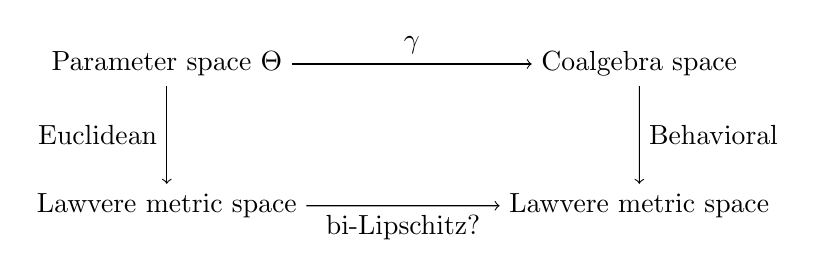
\begin{tikzpicture}[scale=1.2]
\node (Theta) at (0, 0) {Parameter space $\Theta$};
\node (Coalg) at (5, 0) {Coalgebra space};
\node (LTheta) at (0, -1.5) {Lawvere metric space};
\node (LCoalg) at (5, -1.5) {Lawvere metric space};

\draw[->] (Theta) -- node[above] {$\gamma$} (Coalg);
\draw[->] (Theta) -- node[left] {Euclidean} (LTheta);
\draw[->] (Coalg) -- node[right] {Behavioral} (LCoalg);
\draw[->] (LTheta) -- node[below] {bi-Lipschitz?} (LCoalg);
\end{tikzpicture}
\end{center}

Distance matching asks: is the bottom arrow bi-Lipschitz?

\section{Connection to Semiring Relaxation}

This framework connects Part II and Part III:

\subsection{Why Semiring Relaxation Helps}

In Part II, we softened discrete coalgebras to semiring-valued coalgebras to enable gradient descent.

Now we see another benefit: \textbf{softening makes behavioral distance continuous}.

\begin{itemize}
    \item Hard DFA: small parameter change can cause discrete behavior jump (0 $\to$ 1)
    \item Soft DFA: parameter change causes proportional behavior change
\end{itemize}

Softening is necessary not just for gradients, but for distance matching!

\subsection{The Full Picture}

\begin{enumerate}
    \item \textbf{Part I}: Define the structure (coalgebra, bisimulation)
    \item \textbf{Part II}: Soften to enable gradients (semiring relaxation)
    \item \textbf{Part III}: Parameterize to match distances (behavioral metric)
\end{enumerate}

Together: a principled pipeline from structure to learnable system.

\section{Implications}

If this framework is correct:

\begin{keyinsight}
Architecture design becomes \textbf{geometry matching}:
\begin{enumerate}
    \item Compute the behavioral metric of your target coalgebra class
    \item Construct a parameter space with matching metric geometry
    \item Gradient descent then ``does the right thing''
\end{enumerate}
This is no longer alchemy. It is engineering from first principles.
\end{keyinsight}

\section{Open Problems}

\begin{enumerate}
    \item \textbf{Compute behavioral metrics}: For specific functors (DFA, Markov, Kripke), what is the behavioral metric explicitly?

    \item \textbf{Construct matching parameterizations}: Given a behavioral metric, how to design $\Theta$ to match it?

    \item \textbf{Verify known architectures}: Do successful architectures (CNN, ResNet, Transformer) achieve approximate distance matching? Can we measure this?

    \item \textbf{Generalization}: Distance matching addresses optimization. Does it also help generalization?

    \item \textbf{Approximation}: When perfect matching is impossible, what's the best approximation? Is there a canonical ``closest'' parameterization?
\end{enumerate}

These are the questions for future research.
